\section{Experiments}
\label{sec:expr}

In this section, we first give introduction to the two datasets we used to test our model; 
and then introduced the details in our implementation in experiments; 
next, we briefly introduce the evaluation metrics and baseline we applied.
We report the experimental results on joint model based geo-localization and saliency estimation in the last two sub-sections, and give some analysis.

\subsection{Datasets}
We use two challenging datasets, Boston Marathon 2013\cite{chen2016boston} and Tokyo Time Machine~\cite{Arandjelovic16}. 
Table ~\ref{table:dataset} shows the summary of the two datasets we used.
\subsubsection{Boston Dataset} 
~Chen et al.~\cite{chen2016boston} collected video clips which are related to the event of Boston Marathon bombing from the internet. 
This is a dataset which focus on a real event. 
In the videos, the streets look very different from daily appearance due to the event.
Figure~\ref{fig:bostonvideo} shows some example videos. 
In this dataset, they also provide $10,000$ satellite environment images in the surrounding region of the event location. 
The region contains $562$ buildings in total. 
We uniformly sampled 2,500 GPS locations in this region. 
For each GPS coordinate, we collected 4 images from 4 different perspectives of view (10,000 images in total).
We also collected the same number of images as queries for training at randomly sampled GPS locations in the same way to collect database.
For testing, we labeled the ground truth of geo-location for $100$ sampled frames from $37$ 45-degree-view video clips. Some example frames are shown in Figure~\ref{fig:bostonvideo}. Each frame may have multiple relevant images in the database.
\begin{figure}[htbp]
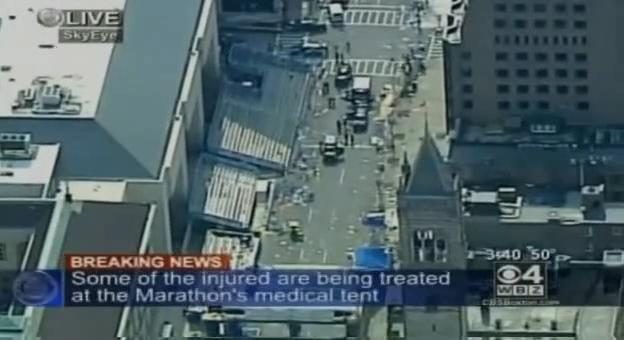
\includegraphics[width=0.4\linewidth]{img/video_1}
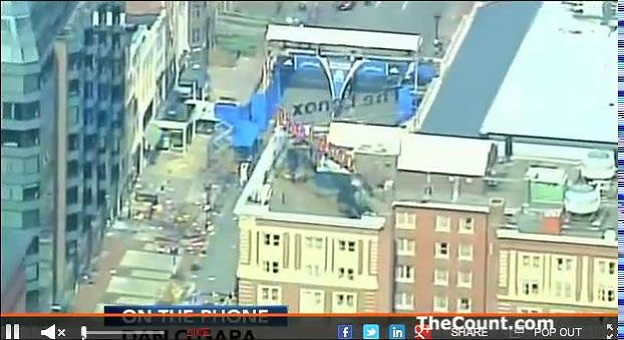
\includegraphics[width=0.4\linewidth]{img/video_2}
\\[0.1cm]
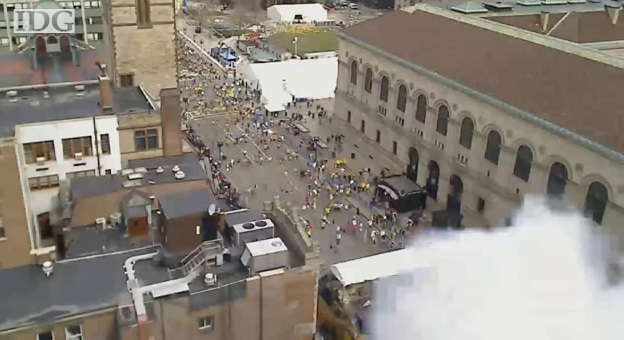
\includegraphics[width=0.4\linewidth]{img/video_3}
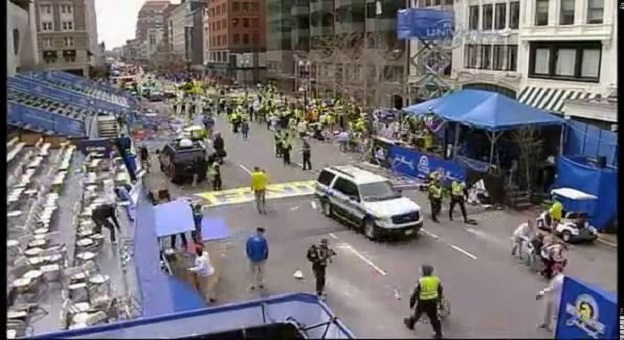
\includegraphics[width=0.4\linewidth]{img/video_4}
\caption{Sample video clips collected from the internet.}
\label{fig:bostonvideo}
\end{figure}


\subsubsection{Tokyo Time Machine Dataset} 
~Tokyo Time Machine (TokyoTM) dataset was released by Arandjelovic et al.~\cite{Arandjelovic16}, generated  from  downloaded  Time  Machine  panoramas. 
In this dataset, the appearances of buildings also change a lot, since the pictures were taken at different time in different days.

\begin{table}[htbp]
\begin{tabular}{l|rr}
Dataset & Database & Query set \\
\hline
\hline
Tokyo Time Machine-train & 49,104 & 7,277 \\
Tokyo Time Machine-val & 49,056 & 7,186 \\
Tokyo 24/7 (-test) & 75,984 & 1,125\\
\hline
Boston-train & 8,000 & 8,000 \\
Boston-val & 2,000 & 2,000 \\
Boston-test & 10,000 & 37 video clips
\end{tabular}
\caption{The size of the dataset we used in the experiments. The train/val(idation)/test dataset is mutually disjoint geographically.}
\label{table:dataset}
\end{table}


\subsection{Implementation Details}
In the following experiments, we use Caffe~\cite{jia2014caffe} as the deep learning framework.

We divide an image into a ``pyramid'', where the first layer is the image itself, the second layer contains $2 \times 2$ sub-images and the third layer contains $3 \times 3$ sub-images. 
Thus, each image has 14 regions when we apply our saliency guided geo-localization method. The saliency score of each region is estimated separately. 
Figure~\ref{fig:regions} shows how we generate regions for an image in the experiments. 

\begin{figure}[htbp]
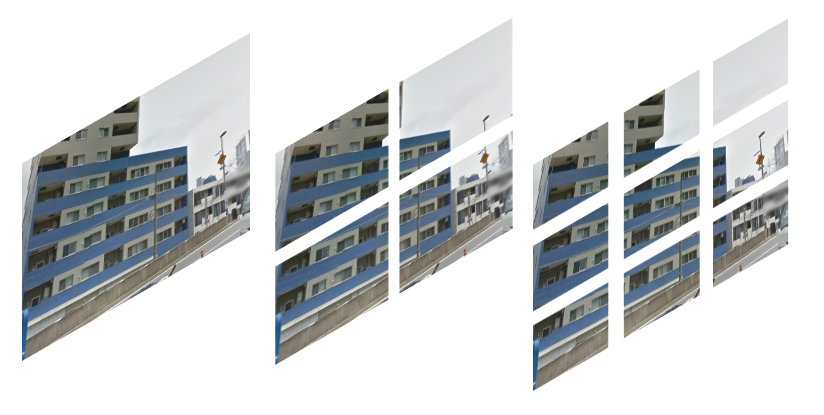
\includegraphics[width=0.8\linewidth]{img/regions}
\caption{The regions of an image in our experiments.}
\label{fig:regions}
\end{figure}

To compare with Eq~\eqref{eq:simR}, we also report the experimental results with another metric of similarity
\begin{equation} 
sim(q, d) =  -||f(q) - f(d)||_2
\label{eq:sim}
\end{equation}
which is directly the additional inverse of the Euclidean distance between two representative vectors in the feature space. 

\subsection{Evaluation Metrics and Baselines}
We test the performance of our model with adopting two common metrics: mean average precision (MAP) and recall on top$N$:\\
1. \emph{MAP} For a query image, the average precision of an image retrieval task can be computed by $AveP=\frac{\sum_{k=1}^nP(k)\times rel(k)}{number~of~relevant~images}$, where $P(k)$ is the precision at cut-off $k$ in the list; $rel(k)$ is an indicator function equalling $1$ if the image at rank $k$ is a relevant image, $0$ otherwise. Then $MAP=\frac{\sum_{i=1}^{|Q|}AveP(i)}{|Q|}$, where $|Q|$ is the number of queries. This metric shows the general performance for a model. \\
2. \emph{Recall on Top $N$.} We retrieve $N$ most similar images for each query. Therefore $Recall on top N = \frac{\sum_{i=1}^{|Q|} \#RetrievedRelevantImage(i)}{\sum_{i=1}^{|Q|} \# RelevantImage(i)}$, where $\#$ represents number. This metric is helpful to reveal the application value for a method, since we often retrieve top $N$ images for image retrieval tasks, like geo-localization.

We applied our method introduced in Section~\ref{sec:solution} with VGG-CNN-M model as a base CNN model and we introduce the following baselines:
\begin{itemize}
\item VGG-CNN-M-$sim$: it calculates similarity $sim$ by Eq~\eqref{eq:sim} using the $fc7$ layer output of the model released by Chatfield et al.~\cite{chatfield2014return}. 
\item VGG-CNN-M-$sim_R$: it estimates the saliency score using the VGG-CNN-M model, and then compute the similarity between image $q$ and $d$ by Eq~\eqref{eq:simR}. 
\item IBFT-$sim$: it applies image-level based fine-tuning to the matching model, and use Eq~\eqref{eq:sim} as the metric of similarity. 
\item JSEM-$sim_R$: it is the full joint saliency estimation and matching model with the similarity measurement Eq~\eqref{eq:simR} proposed in this paper. 
\item Manually-labeled-$sim_R$: For Boston dataset, we also manually label the building contour in the image using LabelMe~\cite{Russell2008}. 
We treat building areas as foreground and other areas as background. 
We manually set the saliency value of a region based on its intersection percentage with the foreground, and use this saliency value from additional building contour labeling in similarity measurement $sim_R$. It could be treated as a kind of upper bound. 
\end{itemize}

\subsection{Evaluation of Geo-Localization}
\begin{table}[htbp]
\begin{tabular}{|l|l|l|}
\hline
Model & Boston & Tokyo TM\\
\hline \hline
VGG-CNN-M-$sim$ & 28.85 & 26.83\\
VGG-CNN-M-$sim_R$ & 35.67 & 24.34\\
IBFT-$sim$ & 37.50 & 23.91\\
JSEM-$sim_R$ & \textbf{58.33} & \textbf{37.01}\\
Manually-labeled-$sim_R$ & 63.40 & -\\
\hline
\end{tabular}
\caption{MAP $(\times 100)$ on the two datasets.}
\label{table:map}
\end{table}

\begin{table}[htbp]
\begin{tabular}{p{0.28\linewidth}|c|c|c|c}
Query Frame & 
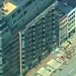
\includegraphics[width=0.13\linewidth]{img/case_1} &
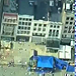
\includegraphics[width=0.13\linewidth]{img/case_2} &
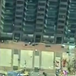
\includegraphics[width=0.13\linewidth]{img/case_3} &
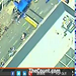
\includegraphics[width=0.13\linewidth]{img/case_4} \\
Ground Truth & 
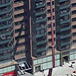
\includegraphics[width=0.13\linewidth]{img/case_1_grnd} &
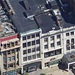
\includegraphics[width=0.13\linewidth]{img/case_2_grnd} &
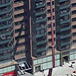
\includegraphics[width=0.13\linewidth]{img/case_3_grnd} &
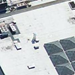
\includegraphics[width=0.13\linewidth]{img/case_4_grnd} \\
\hline
\multicolumn{5}{l}{\textbf{Ground Truth Ranking in All Database Images}} \\
\hline
VGG-CNN-M-$sim$ & 6 & 3 & 10 & 108\\
JSEM-$sim_R$ & 1 & 1 & 1 & 12\\
\end{tabular}
\caption{Case study on Boston Dataset.}
\label{table:bostoncase}
\end{table}

\begin{table*}[h]
\begin{tabular}{l|l|l|l|l|l|l|l|l|l}
\textbf{Model} & \textbf{N = 1} & \textbf{N = 2}& \textbf{N = 3}& \textbf{N = 4}& \textbf{N = 5}& \textbf{N = 10}& \textbf{N = 15} & \textbf{N = 20} & \textbf{N = 25} \\
\hline
VGG-CNN-M-$sim$ &7.05 & 13.85 & 21.41 & 25.44 & 30.23 & 44.33 & 51.89 & 62.97 & 69.77 \\
VGG-CNN-M-$sim_R$ & 8.31 & 15.87 & 23.43 & 30.23 & 35.52 & 53.40 & 73.05 & 80.35 & 84.13 \\
IBFT-$sim$ & 7.56 & 15.62 & 23.93 & 37.03 & 42.82 & 56.93 & 67.25 & 78.84 & 85.89 \\
JSEM-$sim_R$ & 16.12 & 27.96 & 39.80 & 51.39 & 58.44 & 78.84 & 84.63 & 89.67 & 95.21
\end{tabular}
\caption{Recall on top $N$ on Boston dataset.}
\label{table:boston_recall}
\end{table*} 


\begin{table*}[h]
\begin{tabular}{l|l|l|l|l|l|l|l|l|l}
\textbf{Model} & \textbf{N = 1} & \textbf{N = 2}& \textbf{N = 3}& \textbf{N = 4}& \textbf{N = 5}& \textbf{N = 10}& \textbf{N = 15} & \textbf{N = 20} & \textbf{N = 25} \\
\hline
VGG-CNN-M-$sim$ & 5.67&10.17& 14.42& 17.97& 20.33& 32.86& 46.57& 58.16& 68.32 \\
VGG-CNN-M-$sim_R$ & 5.91& 10.87& 15.84& 18.68& 21.04& 36.17& 47.28& 61.47& 70.92 \\
IBFT-$sim$ & 7.57& 11.58& 15.60& 18.91& 23.17& 34.04& 46.57& 55.79& 68.09 \\
JSEM-$sim_R$ & 9.22 & 15.60 & 21.28 & 25.77& 28.84&48.70&63.83&74.23&84.87 
\end{tabular}
\caption{Recall on Top $N$ on Tokyo TM dataset.}
\label{table:netvlad-result}
\end{table*} 

\begin{figure*}[h]
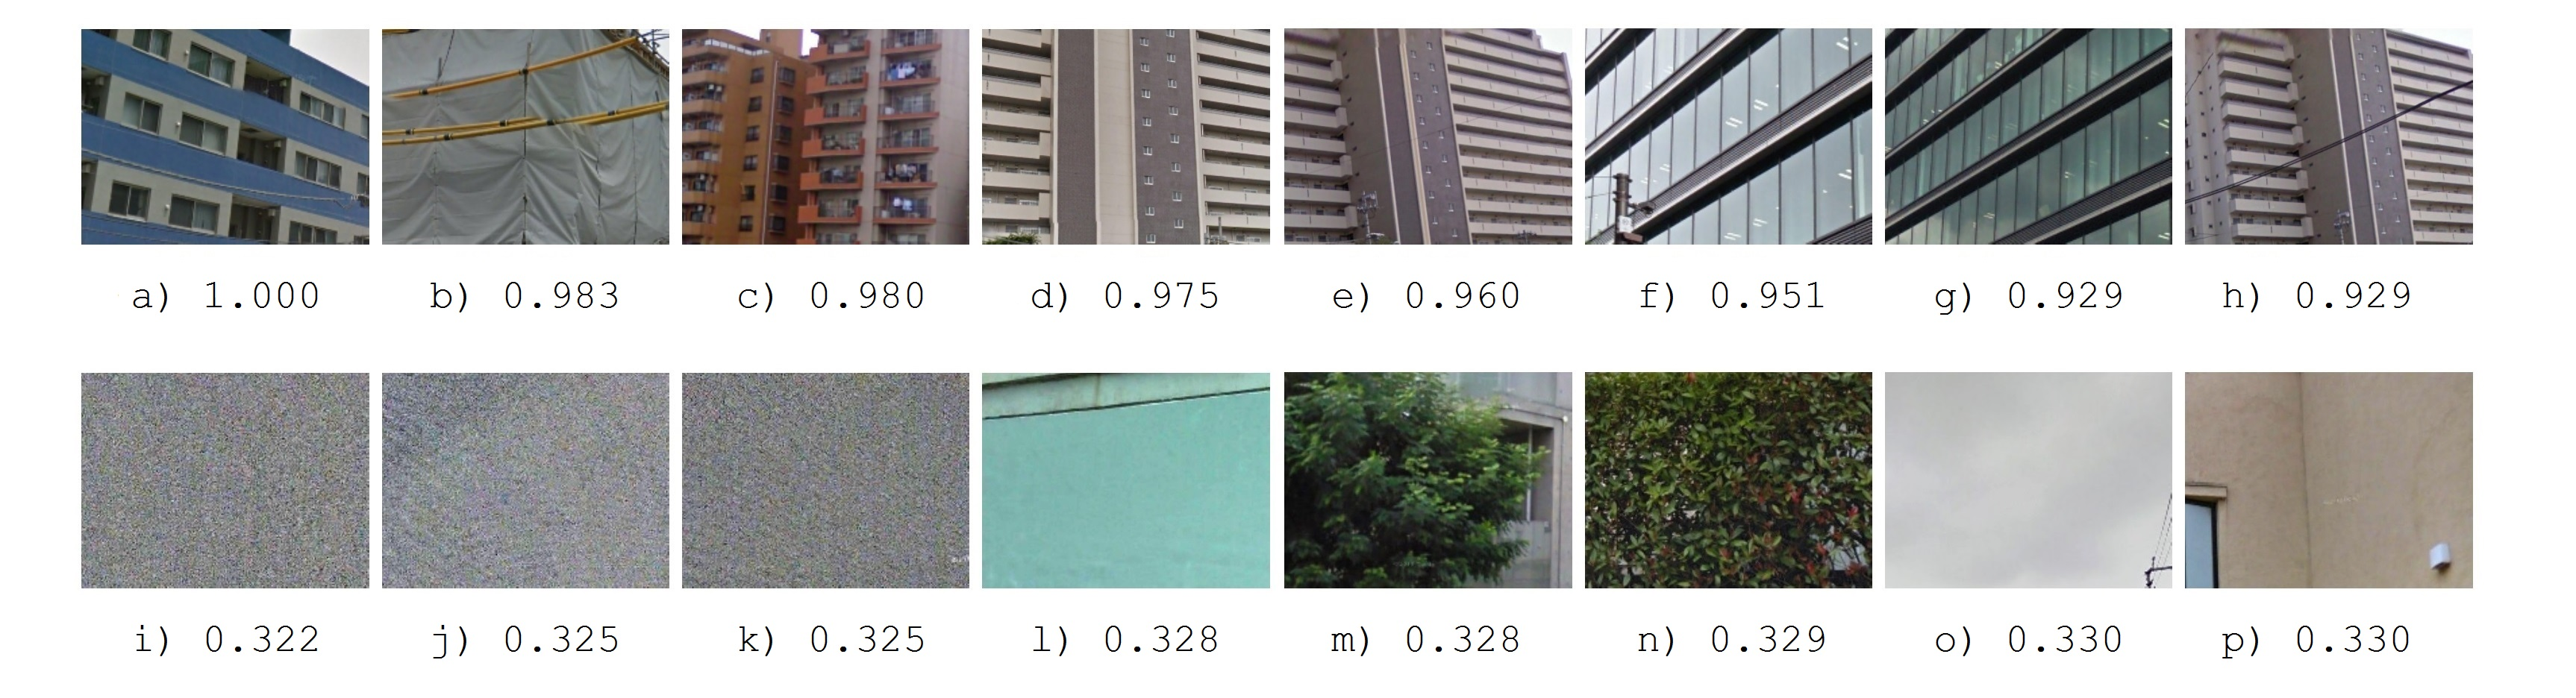
\includegraphics[width=0.9\textwidth]{img/salient}
\caption{8 most salient regions(top) and 8 most non-salient regions in Tokyo TM database, with their saliency score.}
\label{fig:saliency}
\end{figure*}

\emph{Boston: }
The result reported in Table~\ref{table:map} shows that our model has significantly improved the mean average precision (MAP) on the geo-localization task. For the convenience of view, Table~\ref{table:bostoncase} shows some case study on this task, from which we can easily see that the rankings of ground truth images raise a lot. In CNN, we resize the frames into a $224 \times 224$ square shape. Thus, we show the frames and database in such square shapes rather than rectangular ones in Figure~\ref{fig:bostonvideo}. Besides, the ``recall on top $K$'' result on Boston dataset is reported in Table~\ref{table:boston_recall}.

\emph{TokyoTM: }
We also run experiments on the Tokyo TM dataset and show results in Table~\ref{table:map} and Table~\ref{table:netvlad-result}. 

The experimental result had proved the efficiency of our model, showing that our model obtains the best recall for every $N$, and beats the baselines on the metric MAP. That is, our model not only performs well generally, but also has application value for real image retrieval tasks. However, it's interesting that the model IBFT-$sim$ performs  similar to VGG-CNN-M-$sim$ on Tokyo TM dataset. It suggests that fine-tuning based only on the limited training dataset could easily cause over-fitting. This also shows that saliency score is an important part to improve the performance of the model, and make the model more robust.

\subsection{Analysis of Learned Saliency}
To give further supporting evidences for the effectiveness of our method, we analyze the learned saliency qualitatively and quantitatively. 
We first conduct case study on some salient and non-salient regions, and then report the Pearson correlation with manually labeled saliency score on some randomly selected samples.

We applied the method introduced in Section~\ref{sec:solution} to estimate the saliency score for each region of a given image. 
Figure~\ref{fig:saliency} shows the 8 most salient and 8 most non-salient regions together with their saliency scores from the Tokyo TM database. 
The salient regions are all buildings with distinctive structure($a-h$) while the non-salient regions are images from road($i-k$), trees($m$ and $n$), sky($o$) and indistinctive building regions($l$ and $p$). 



We also analyze the correlation between learned saliency with saliency calculate from manually labeled building contour in manually-labeled-$sim_R$, which could be treated as ground truth saliency score. 
The Pearson correlation is $0.7625$, showing that our estimated saliency score has strong relation with the ground truth saliency score.
Figure~\ref{fig:saliencycasestudy} shows the case study of our region based saliency estimation on two specific images. 

\begin{figure}
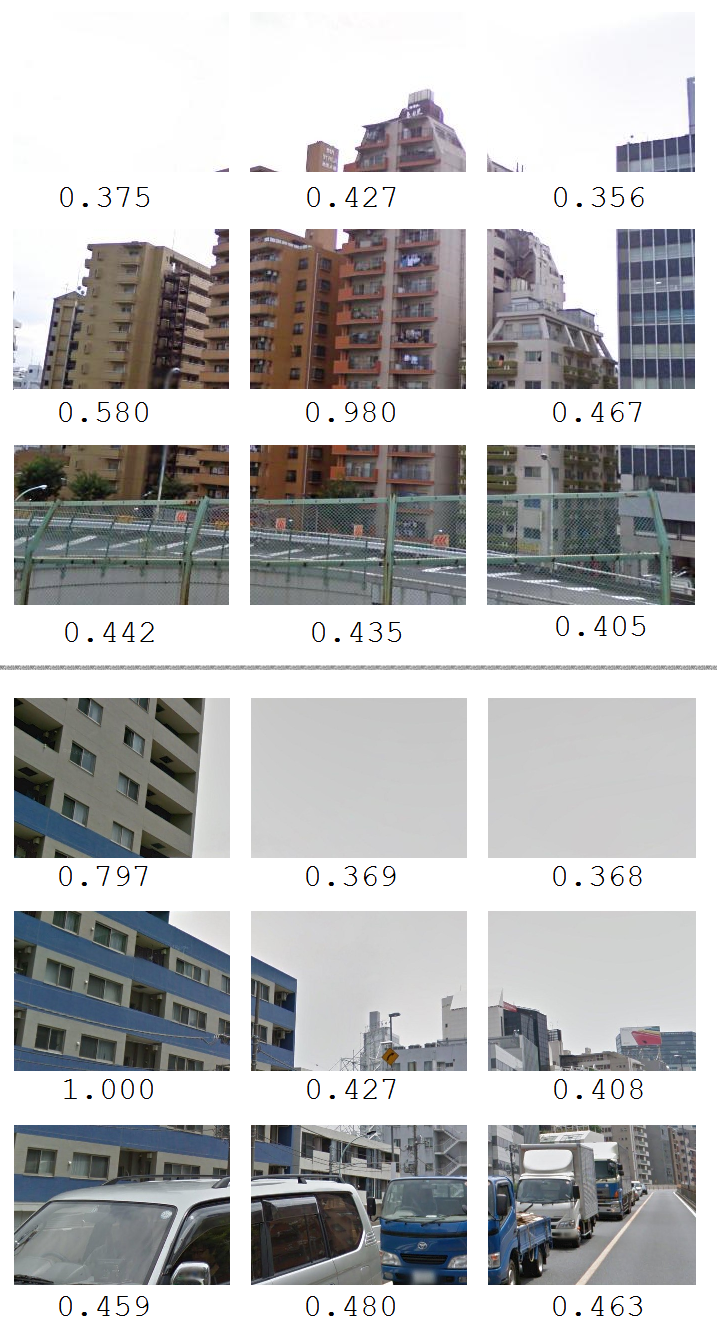
\includegraphics[width=0.73\linewidth]{img/case_study}
\caption{\label{fig:saliencycasestudy}Case study of region-based saliency estimation.}
\end{figure}